\documentclass[usenames,dvipsnames,10pt,aspectratio=169]{beamer} 
% Add option 'aspectratio=169' for 16:9 widescreen 
% Add option  'handout' to ignore animations
% If you have a smaller amount of text, feel free to also try '11pt'! / Jesper

\usepackage[utf8]{inputenc}
\usepackage{verbatim}
\usepackage{minted}
\usemintedstyle{monokai}
\usepackage{graphicx}
\usepackage{wrapfig}
\usepackage[document]{ragged2e}
\usetheme{umu}

\usepackage{hyperref}
\hypersetup{
    colorlinks=true,
    linkcolor=ucuyellow,
    filecolor=ucuyellow,      
    urlcolor=ucuyellow,
}
\urlstyle{same}

%%% Bibliography
\usepackage[style=authoryear,backend=biber]{biblatex}
\addbibresource{bibliography.bib}

\DeclareNameAlias{author}{given-family}

%%% Suppress biblatex annoying warning
\usepackage{silence}
\WarningFilter{biblatex}{Patching footnotes failed}

%%% Some useful commands
% pdf-friendly newline in links
\newcommand{\pdfnewline}{\texorpdfstring{\newline}{ }} 
% Fill the vertical space in a slide (to put text at the bottom)
\newcommand{\framefill}{\vskip0pt plus 1filll}

%%% Enter additional packages below (or above, I can't stop you)! / Jesper
\renewcommand{\proofname}{\sffamily{Proof}}

%%%%%%%%%%%%%%%%%%%%%%%%%%%%%%%%%%%%%%%%%%%%%%%%%%%%%%%%%%%%%%%%%%%%%%%%%%%%%%%%%%%%%
\title[Rust \#2]{Rust \#2: Ownership,\\ Structs and OO}
\date[\today]{\small\today}
\author[Sultanov Andriy]{Sultanov Andriy}
\institute{APPS@UCU}

\begin{document}

\begin{frame}
\titlepage
\end{frame}

\begin{frame}{\contentsname}
\tableofcontents
\end{frame}

\framepic{graphics/1.jpg}{
 \textcolor{ucuwhite}{Error Handling}
 \vskip 0.5cm
 }

\section{Error Handling}

\begin{frame}{Error handling methods}

\inputminted[fontsize=\large]{c}{code/error1.rs}

If you can recover from an error, use an algebraic\\
type Result<T, E>, which can either be\\
Ok(value of type T) or Err(value of type E)
\inputminted[fontsize=\large]{c}{code/error2.rs}
\normalsize

\vskip 0.8cm

\end{frame}

\begin{frame}{Memory layout} 
\inputminted[fontsize=\large]{c}{code/stack.c}
\end{frame}

\begin{frame}{Memory layout} 

\begin{figure}[ht]
	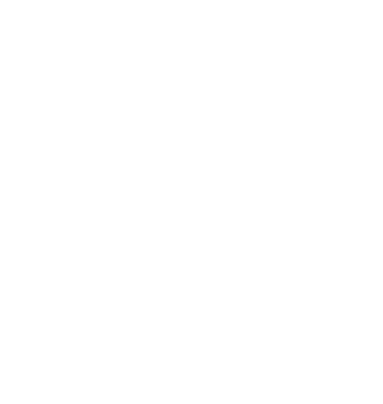
\includegraphics[width=0.4\textwidth]{graphics/stack1.png}
  \hfill
	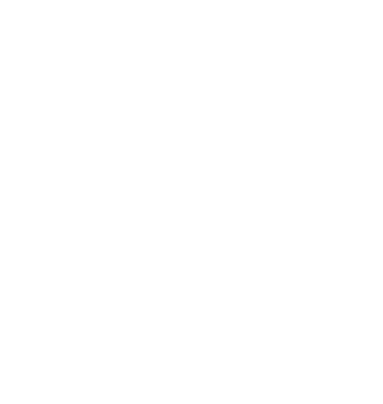
\includegraphics[width=0.4\textwidth]{graphics/stack2.png}
	\hfill
\end{figure}
	
\end{frame}

\end{document}
